\subsection{Constraints}
\label{sec:constraints}

To illustrate the OCL constraints, we provide a partial view of the SDPL UML profile in Figure \ref{fig:sample_profile}\footnote{The attributes of the stereotypes are omitted for simplicity.}.

\begin{figure}[ht!]
	\centering
	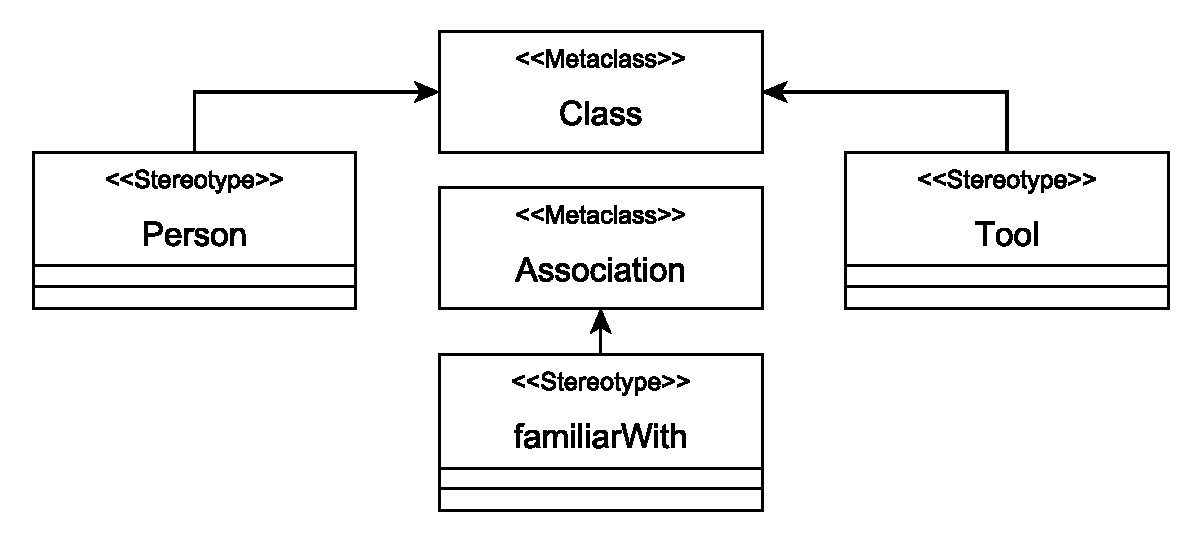
\includegraphics[width=1\textwidth]{diagrams/example_profile}
	\caption[]{Example UML profile for SDPL showing Person, Tool and the familiarWith association}
	\label{fig:sample_profile}
\end{figure}

In Figure \ref{fig:sample_profile}, there are three \emph{Stereotype}s - \emph{Person} and \emph{Tool}, both extend the meta-element \emph{UML::Class}, and they correspond to classes \emph{Person} and \emph{Tool} in the Emfatic code in Listing \ref{lst:annotatedSdplEmfatic}. 
\emph{Stereotype} \emph{familiarWith}, which extends meta-element \emph{UML::Association}, corresponds to the reference \emph{familiarWith} in the \emph{Person} class in Listing \ref{lst:annotatedSdplEmfatic}.

%
%\begin{figure}[ht!]
%	\centering
%	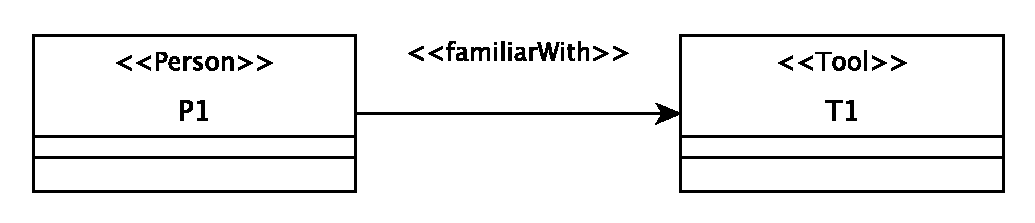
\includegraphics[width=0.5\textwidth]{diagrams/example_class_diagram}
%	\caption[]{Example Class diagram using SDPL UML Profile}
%	\label{fig:sample_class}
%\end{figure}

In Figure~\ref{fig:sdplEditor}, the \textit{familiarWith} association is used to connect \textit{Person} \emph{Alice} with \textit{Tool} \emph{StarUML}. 
However, the \emph{familiarWith} stereotype can be applied to any \emph{Association}, and not strictly to \emph{Associations} which connect \emph{Person} and \emph{Tool} stereotyped elements. 
Therefore, constraints are needed to check (at least) two aspects:

\begin{itemize}
	\item \textbf{End Types}: the elements that a \emph{familiarWith} association connects to that have \emph{Person} and \emph{Tool} stereotypes applied to them;
	\item \textbf{Navigability}: the \emph{familiarWith} association starts from an element stereotyped as \emph{Person} and points to an element stereotyped as \emph{Tool}.
\end{itemize}

\subsubsection{End Types}
Listing \ref{lst:endTypes} shows the OCL code for the \emph{End Types} constraint. 
Line 1 accesses the types that \emph{familiarWith} connects. 
Lines 3 and 4 check if the types that \emph{familiarWith} connects are of type that either has stereotype \emph{Person} or \emph{Tool}. 
In this way, if a \emph{familiarWith} association connects two types that are not \emph{Person} or \emph{Tool}, the constraint fails.

%In UML profiling, meta-element extensions are associations (instead of generalisations)

\lstinputlisting[caption={The End Types constraint in OCL},label={lst:endTypes}, captionpos=b, language=OCL, tabsize=2, numbers=left, numbersep=5pt, numberstyle=\tiny, breaklines=true, escapeinside={(*}{*)}]{endtypes.txt}

\subsubsection{Navigability}
Listing \ref{lst:navigability} shows the OCL code for the \emph{Navigability} constraint. 
In this case, we are interested in checking the \emph{isNavigable} property of each end. 
Thus, in lines 2 and 3, we obtain the member ends that \emph{familiarWith} connects with. 
If these ends are obtained successfully (line 4), we check that the \emph{personEnd} (connecting element stereotyped as \emph{Person}) is not navigable (line 5) and the \emph{toolEnd} (connecting element stereotyped as \emph{Tool}) is navigable (line 6). 
Therefore, we are checking that a \emph{familiarWith} association can only go from \emph{Person} to \emph{Tool} and not the other way around. 
We need to highlight, that currently, opposite references are not supported; plans for future work are outlined in Section~\ref{sec:future}.

\begin{figure}[h]
	\lstinputlisting[caption={The Navigability constraint in 
		OCL},label={lst:navigability}, captionpos=b, language=OCL, tabsize=2, 
	numbers=left, numbersep=5pt, numberstyle=\tiny, breaklines=true, 
	escapeinside={(*}{*)}]{navigability.txt}
	
	\vspace*{-5mm}
\end{figure}

With these two constraints implemented, we are able to automatically generate OCL constraints for stereotypes that extend \emph{UML::Association}. 
We use the \emph{End Types} and \emph{Navigability} constraints as templates with dynamic sections (where the specific stereotype names are inserted dynamically, e.g., \emph{Person} and \emph{Tool}). 
So far we have only explored stereotypes that extend \emph{UML::Association}. 
The constraint templates for stereotypes that extend other UML relationships need to be developed separately as the means to 
access source/target elements of the relationship are different.


